
\documentclass[template=tabling,81pt,headonall]{azmoon}
\usepackage{xepersian}
\usepackage{amsfonts}
\usepackage{graphicx}
\graphicspath{ {./images/} }
\settextfont{Yas}
\setdigitfont{A Iranian Sans}
\usepackage{fontawesome5}

\printanswers
    \teacher{محمد صالح علی اکبری}
    \teachertitle{دبیر}
    \city{گناباد}
    \schooltitle{متوسطه دوره دوم}
    \school{شاهد امام (ره)}
    \grade{دهم}
    \branch{۱۵۱}
    \topic{ریاضی}
    \examdate{آذر ۱۴۰۲}
    \answertime{80 دقیقه}
    \begin{document}
	\begin{questions}
		\nointerlineskip%
		\vskip-\baselineskip
		\question[1]{%
ناحیه رنگی در نمودار ون مقابل، کدام مجموعه را مشخص می‌کند؟ \\ 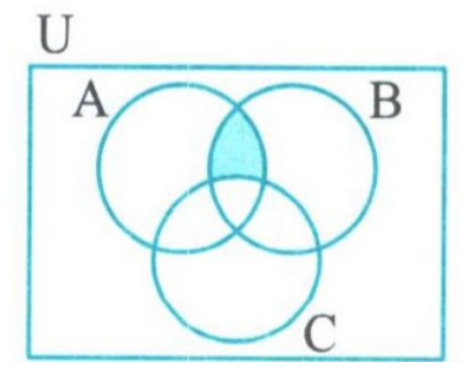
\includegraphics[scale = 0.18]{Screenshot from 2023-12-15 04-49-09}
    \begin{fourchoice}[4]\choice{$(A\bigcup B) \bigcap C'$}
\choice{$A\bigcap (B\bigcup C)'$}
\choice{$A\bigcap(B-C)'$}
\choice{$(A\bigcap B)\bigcap C'$}
\end{fourchoice}

            }\question[1]{%
اگر مجموعه مرجع $\mathbb{R}$ باشد، $A = [2 , 5]$ و $B = (4 , 8)$، مجموعه $B'-A'$ کدام است؟
    \begin{fourchoice}[1]\choice{$(2,4]$}
\choice{$[2,4]$}
\choice{$[2,4]\bigcup[5,8]$}
\choice{$[2,4]\bigcup(5,8)$}
\end{fourchoice}

            }\question[1]{%
مقدار عبارت $A=\dfrac{\tan^2 30^\circ + \tan^245^\circ + \tan^2 60^\circ }{\cot60^\circ -\cot30^\circ}$ کدام است؟
    \begin{fourchoice}[4]\choice{$\dfrac{13\sqrt{3}}{6}$}
\choice{$-\dfrac {13\sqrt {3}}{6}$}
\choice{$-2\sqrt{3}$}
\choice{$2\sqrt{3}$}
\end{fourchoice}

            }\question[1]{%
در شکل مقابل، طول طناب ABC بر حسب $\theta$ کدام است؟ \\ 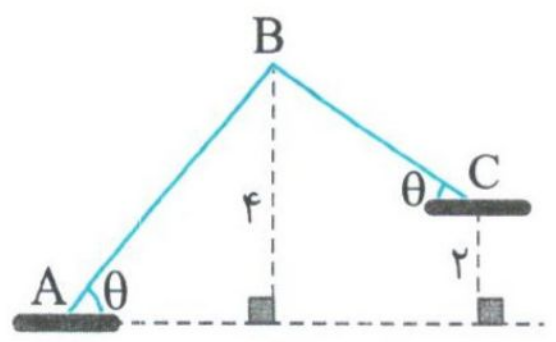
\includegraphics[scale = 0.18]{Screenshot from 2023-12-15 06-07-16}
    \begin{fourchoice}[4]\choice{$\dfrac{8}{\cos\theta}$}
\choice{$\dfrac{2}{\cos\theta}$}
\choice{$\dfrac{6}{\sin\theta}$}
\choice{$\dfrac{3}{sin \theta}$}
\end{fourchoice}

            }\question[1]{%
در شکل زیر، حاصل $\tan\alpha$ کدام است؟ \\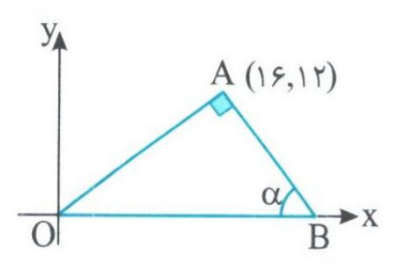
\includegraphics[scale = 0.3]{Screenshot from 2023-12-15 20-26-50}
    \begin{fourchoice}[4]\choice{$\dfrac{5}{3}$}
\choice{$\dfrac{4}{7}$}
\choice{$\dfrac{4}{3}$}
\choice{$\dfrac{3}{8}$}
\end{fourchoice}

            }\question[1]{%
در شکل مقابل مربع‌های کوچک برابرند. مقدار $\tan(x) \tan(y) \tan(z)$ کدام است؟ \\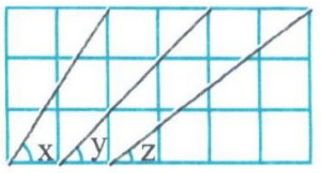
\includegraphics[scale = 0.35]{Screenshot from 2023-12-15 20-31-25}
    \begin{fourchoice}[4]\choice{$1$}
\choice{$\dfrac{9}{8}$}
\choice{$\dfrac{27}{16}$}
\choice{$\dfrac{27}{8}$}
\end{fourchoice}

            }\question[1]{%
مجموع پنج عدد که جملات متوالی دنباله‌ای هندسی هستند برابر ۲ است. اگر عدد وسطی برابر ۱ باشد، مجموع معکوسات این اعداد کدام است؟
    \begin{fourchoice}[4]\choice{$2$}
\choice{$\dfrac{1}{4}$}
\choice{$\dfrac{1}{2}$}
\choice{$1$}
\end{fourchoice}

            }\question[1]{%
در شکل مقابل طول ضلع مربع‌های کوچک برابر ۱ است. مقدار $\cos \beta +\sin \alpha$ کدام است؟ \\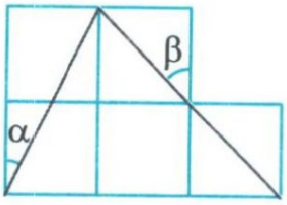
\includegraphics[scale = 0.31]{Screenshot from 2023-12-15 20-36-57}
    \begin{fourchoice}[4]\choice{$\dfrac{\sqrt{2}+ \sqrt{5}}{\sqrt{10}}$}
\choice{$\dfrac{1+\sqrt{5}}{\sqrt{10}}$}
\choice{$\dfrac{1+\sqrt{2}}{\sqrt{10}}$}
\choice{$\dfrac{\sqrt{2}+\sqrt{3}}{\sqrt{10}}$}
\end{fourchoice}

            }\question[1]{%
در شکل زیر از بالای یک فانوس دریایی به ارتفاع $200$ متر، یک قایق با زاویه $35^{\circ}$ و قایق دیگری با زاویه $27^{\circ}$ دیده می‌شود. فاصله دو قایق از یکدیگر چقدر است؟ ($\tan 35^{\circ} = 0.7$ و $\tan 27^{\circ} = 0.5$)\\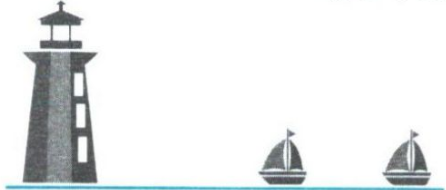
\includegraphics[scale = 0.3]{Screenshot from 2023-12-15 20-45-31}
    \begin{fourchoice}[4]\choice{$30$}
\choice{$40$}
\choice{$20$}
\choice{$50$}
\end{fourchoice}

            }\question[1]{%
در شکل مقابل $\hat{A}= 90^{\circ}، \widehat{ABD}=\widehat{DBC}=30^\circ$ و $AD = 12$. طول $DC$ چقدر است؟ \\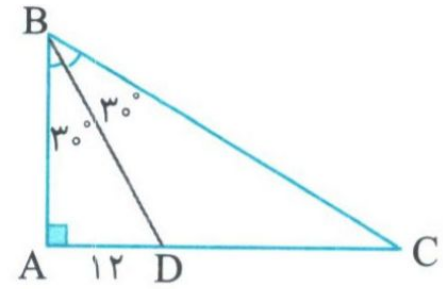
\includegraphics[scale = 0.31]{Screenshot from 2023-12-15 21-00-26}
    \begin{fourchoice}[4]\choice{$18$}
\choice{$20$}
\choice{$24$}
\choice{$15$}
\end{fourchoice}

            }\question[1]{%
اگر $[-1 , 5) \bigcap [a,6) = [2a-1 , 5)$، در بازه $[-a , a]$ چند عدد صحیح وجود دارد؟
    \begin{fourchoice}[4]\choice{$4$}
\choice{$3$}
\choice{$2$}
\choice{$1$}
\end{fourchoice}

            }\question[1]{%
در شکل مقابل طول ضلع مربع‌های کوچک برابر ۱ است. مقدار $\cos \alpha$ کدام است؟ \\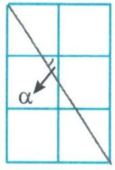
\includegraphics[scale = 0.7]{Screenshot from 2023-12-15 21-07-51}
    \begin{fourchoice}[4]\choice{$\dfrac{2}{\sqrt{13}}$}
\choice{$\dfrac{1}{\sqrt{13}}$}
\choice{$\dfrac{2}{\sqrt{11}}$}
\choice{$\dfrac{1}{\sqrt{11}}$}
\end{fourchoice}

            }\question[1]{%
در شکل زیر طول ضلع HC چقدر است؟ \\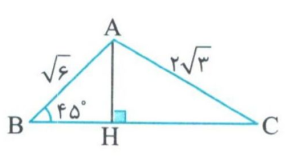
\includegraphics[scale = 0.7]{Screenshot from 2023-12-15 21-16-17}
    \begin{fourchoice}[4]\choice{$\sqrt{3}$}
\choice{$\dfrac{1}{\sqrt{13}}$}
\choice{$\dfrac{2}{\sqrt{11}}$}
\choice{$\dfrac{1}{\sqrt{11}}$}
\end{fourchoice}

            }\question[1]{%
در شکل مقابل $ABCD$ مستطیل است، $DE=4$ و $BC=5$. مقدار $\cot \alpha$ کدام است؟ \\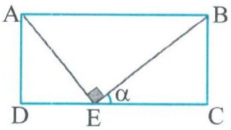
\includegraphics[scale = 0.651]{Screenshot from 2023-12-15 21-16-33}
    \begin{fourchoice}[4]\choice{$\dfrac{4}{5}$}
\choice{$\dfrac{5}{4}$}
\choice{$\dfrac{4}{3}$}
\choice{$\dfrac{3}{4}$}
\end{fourchoice}

            }\question[1]{%
در شکل مقابل مساحت مثلث ABC کدام است؟ \\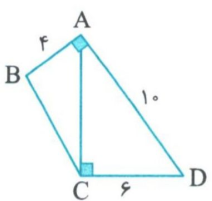
\includegraphics[scale = 0.65]{Screenshot from 2023-12-15 21-16-50}
    \begin{fourchoice}[4]\choice{$\dfrac{64}{5}$}
\choice{$\dfrac{64}{3}$}
\choice{$\dfrac{64}{9}$}
\choice{$\dfrac{64}{7}$}
\end{fourchoice}

            }\question[1]{%
کدام است؟ $\dfrac{x^2+x+1}{2x^2+5x}\div\dfrac{x^3-1}{2x^2+3x-5}$
    \begin{fourchoice}[4]\choice{$\dfrac{2}{1+x}$}
\choice{$\dfrac{1}{2-x}$}
\choice{$x$}
\choice{$\dfrac{1}{x}$}
\end{fourchoice}

            }\question[1]{%
اگر $ab=1$ و $a-b=76$ مقدار $\sqrt[3]{a} - \sqrt[3]{b}$ کدام است؟
    \begin{fourchoice}[4]\choice{$3$}
\choice{$4$}
\choice{$5$}
\choice{$6$}
\end{fourchoice}

            }\question[1]{%
معکوس عدد$\sqrt{2-\sqrt{2}}$برابر کدام است؟
    \begin{fourchoice}[4]\choice{$\sqrt{4+\sqrt{2}}$}
\choice{$\sqrt{1+\dfrac{\sqrt{2}}{2}}$}
\choice{$\sqrt{\sqrt{2}+1}$}
\choice{$\sqrt{\sqrt{2}-1}$}
\end{fourchoice}

            }\question[1]{%
حاصل $\dfrac{4+2\sqrt{3}}{\sqrt{3}-1}-5$ را محاسبه کنید.}\question[2]{%
اگر $\dfrac{1}{\sqrt[3]{3}-1} = \dfrac{1}{2}\sqrt[3]{9}+\dfrac{1}{2}\sqrt[3]{3}+a$ مقدار a را محاسبه کنید.}\question[1]{%
حاصل عبارت $A=\dfrac{\sqrt{2+\sqrt{3}}+\sqrt{2-\sqrt{3}}}{\sqrt{2+\sqrt{3}}-\sqrt{2-\sqrt{3}}}$}\end{questions}
    \end{document}
    